%%%%%%%%%%%%%%%%%%%%%%%%%%%%%%%%%%%%%%%%%%%%%%%%%%%%%%%%%%%%%%%%%%%%%%%%

%%% LaTeX Template for ECAI Papers 
%%% Prepared by Ulle Endriss (version 1.0 of 2023-12-10)

%%% To be used with the ECAI class file ecai.cls.
%%% You also will need a bibliography file (such as mybibfile.bib).

%%%%%%%%%%%%%%%%%%%%%%%%%%%%%%%%%%%%%%%%%%%%%%%%%%%%%%%%%%%%%%%%%%%%%%%%

%%% Start your document with the \documentclass{} command.
%%% Use the first variant for the camera-ready paper.
%%% Use the second variant for submission (for double-blind reviewing).

\documentclass{ecai} 
%\documentclass[doubleblind]{ecai} 

%%%%%%%%%%%%%%%%%%%%%%%%%%%%%%%%%%%%%%%%%%%%%%%%%%%%%%%%%%%%%%%%%%%%%%%%

%%% Load any packages you require here. 

\usepackage{latexsym}
\usepackage{appendix}
\usepackage{amssymb}
\usepackage{amsmath}
\usepackage{amsthm}
\usepackage{booktabs}
\usepackage{enumitem}
\usepackage{graphicx}
\usepackage{color}
\usepackage{tikz}
\usetikzlibrary{shapes.geometric, arrows.meta, positioning, fit, backgrounds, calc}
\usepackage{tabularx}
\usepackage{xcolor}
\usepackage{float}
\usepackage[colorlinks=true, linkcolor=blue]{hyperref}
\setlength{\emergencystretch}{3em}

%%%%%%%%%%%%%%%%%%%%%%%%%%%%%%%%%%%%%%%%%%%%%%%%%%%%%%%%%%%%%%%%%%%%%%%%

%%% Define any theorem-like environments you require here.

\newtheorem{theorem}{Theorem}
\newtheorem{lemma}[theorem]{Lemma}
\newtheorem{corollary}[theorem]{Corollary}
\newtheorem{proposition}[theorem]{Proposition}
\newtheorem{fact}[theorem]{Fact}
\newtheorem{definition}{Definition}

%%%%%%%%%%%%%%%%%%%%%%%%%%%%%%%%%%%%%%%%%%%%%%%%%%%%%%%%%%%%%%%%%%%%%%%%

%%% Define any new commands you require here.

\newcommand{\BibTeX}{B\kern-.05em{\sc i\kern-.025em b}\kern-.08em\TeX}

%%%%%%%%%%%%%%%%%%%%%%%%%%%%%%%%%%%%%%%%%%%%%%%%%%%%%%%%%%%%%%%%%%%%%%%%

\begin{document}

%%%%%%%%%%%%%%%%%%%%%%%%%%%%%%%%%%%%%%%%%%%%%%%%%%%%%%%%%%%%%%%%%%%%%%%%

\begin{frontmatter}

%%% Use this command to specify your submission number.
%%% In doubleblind mode, it will be printed on the first page.

\paperid{123} 

%%% Use this command to specify the title of your paper.

\title{AI Tutor: An adaptive multi-agent learning system}

%%% Use this combinations of commands to specify all authors of your 
%%% paper. Use \fnms{} and \snm{} to indicate everyone's first names 
%%% and surname. This will help the publisher with indexing the 
%%% proceedings. Please use a reasonable approximation in case your 
%%% name does not neatly split into "first names" and "surname".
%%% Specifying your ORCID digital identifier is optional. 
%%% Use the \thanks{} command to indicate one or more corresponding 
%%% authors and their email address(es). If so desired, you can specify
%%% author contributions using the \footnote{} command.

\author[A]{\fnms{First}~\snm{Author}\orcid{....-....-....-....}\thanks{Corresponding Author. Email: somename@university.edu.}\footnote{Equal contribution.}}
\author[B]{\fnms{Second}~\snm{Author}\orcid{....-....-....-....}\footnotemark}
\author[B,C]{\fnms{Third}~\snm{Author}\orcid{....-....-....-....}} 

\address[A]{Short Affiliation of First Author}
\address[B]{Short Affiliation of Second Author and Third Author}
\address[C]{Short Alternate Affiliation of Third Author}

%%% Use this environment to include an abstract of your paper.

\begin{abstract}
A platform that provides personalised, comprehensive, and adaptive
learning material in a guided manner at a single place is not easily
accessible to many learners who wish to study a topic or resolve
conceptual doubts. While general-purpose LLMs such as GPT models are
widely used for this purpose, they are prone to hallucination and can
introduce further confusion rather than clarity. Existing systems lack
the guardrails, structured feedback mechanisms, and domain grounding
needed to serve as a reliable, end-to-end learning companion.
\textbf{AI Tutor}, a multi-agent backend system for
personalised, adaptive learning. The system is designed in a guided
manner with multiple guardrails, rubrics, and critic-discriminator
components that verify factual correctness and provide a one-stop
solution for learners. 
\end{abstract}

\end{frontmatter}

%%%%%%%%%%%%%%%%%%%%%%%%%%%%%%%%%%%%%%%%%%%%%%%%%%%%%%%%%%%%%%%%%%%%%%%%

\section{Introduction}

\textbf{AI Tutor} employs a hierarchical agent
architecture in which an Orchestrator Agent coordinates three
specialised downstream agents: a Retrieval-Augmented Generation (RAG)
Agent that extracts and scores content from uploaded PDF documents, a
Teaching Agent that synthesises level-adapted explanations, and a Quiz
Agent that generates and evaluates formative assessments. Agents
communicate asynchronously via Apache Kafka, and the Orchestrator's
internal workflow is managed by a LangGraph \texttt{StateGraph} with
interrupt/resume checkpointing. Our design eliminates heavyweight
orchestration frameworks in favour of a thin, deterministic agent loop,
reducing operational complexity without sacrificing extensibility..


%%%%%%%%%%%%%%%%%%%%%%%%%%%%%%%%%%%%%%%%%%%%%%%%%%%%%%%%%%%%%%%%%%%%%%%%
\section{System Architecture}

\subsection{Overview}
AI Tutor is composed of four independent agents running as
separate pod. Since GraphState can not be shared for agents deployed under different pods, Inter-agent state shared is mediated exclusively
by Apache Kafka, ensuring loose coupling and
horizontal scalability. 
A user session begins when the frontend publishes a
\texttt{PlannerRequestEvent} to the \texttt{init-planner} topic, carrying
the user's natural-language query, optional uploaded PDF paths, and an
optional self-declared learner level. The Orchestrator Worker consumes
this event and drives the remainder of the session.

\begin{figure}[H]
    \centering
    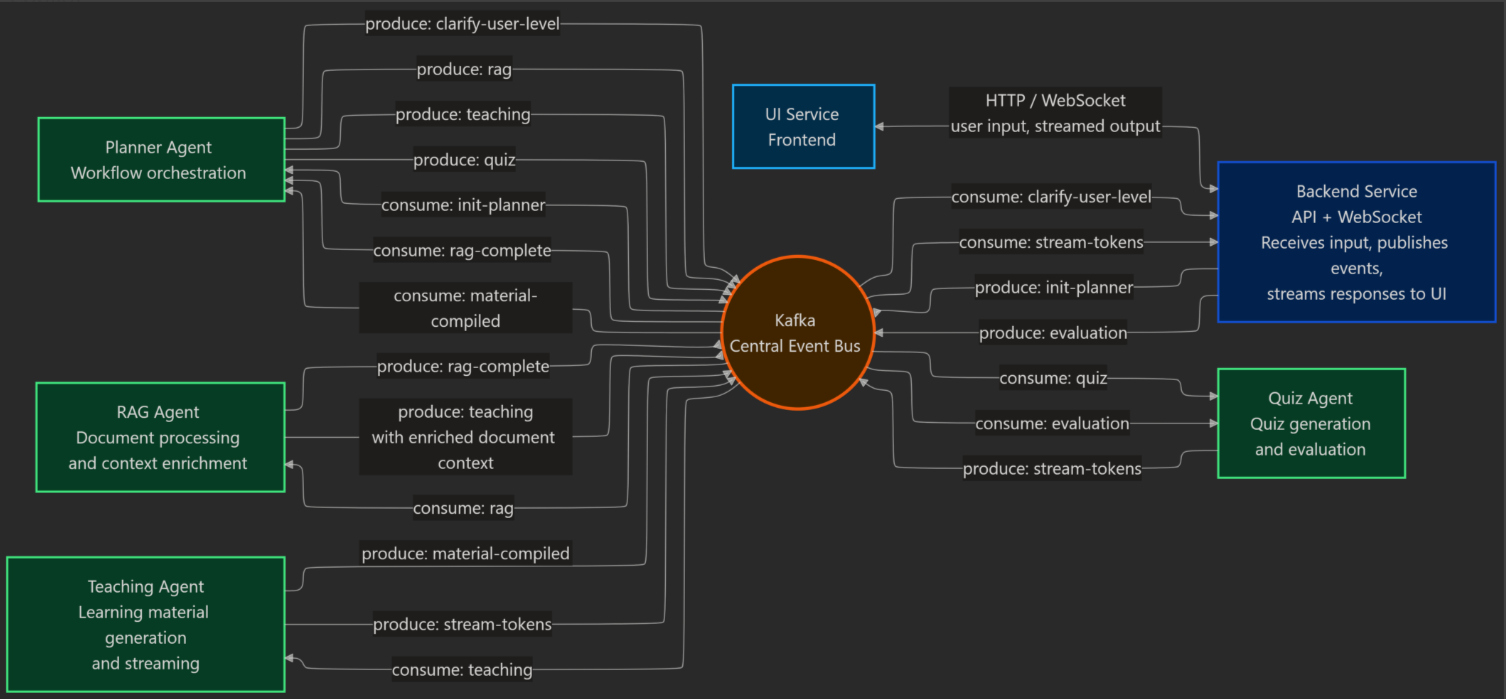
\includegraphics[width=\columnwidth, keepaspectratio]{arch-ai-tutor1.png}
    \caption{AI Tutor Complete Architecture}
    \label{fig:your-label}
\end{figure}


\subsection{Kafka topic registry}

All topic names are centralised in \texttt{project/topics.py} through a
set of \texttt{str}-typed Python \texttt{Enum} classes (e.g.\
\texttt{PlannerTopics}, \texttt{PlannerInboundTopics}). No topic name is
hard-coded outside this module. Table~\ref{tab:topics} lists the principal
topics.



\begin{table}[H]
\centering
\small
\begin{tabular}{lll}
\toprule
\textbf{Topic} & \textbf{Producer} & \textbf{Consumer} \\
\midrule
\texttt{init-planner}      & Frontend       & Orchestrator   \\
\texttt{rag}               & Orchestrator   & RAG Agent      \\
\texttt{rag-complete}      & RAG Agent      & Orchestrator   \\
\texttt{teaching}          & Orchestrator   & Teaching Agent \\
\texttt{material-compiled} & Teaching Agent & Orchestrator   \\
\texttt{quiz-request}      & Orchestrator   & Quiz Agent     \\
\texttt{quiz-complete}     & Quiz Agent     & Orchestrator   \\
\texttt{workflow-complete} & Orchestrator   & Frontend       \\
\bottomrule
\end{tabular}
\caption{Principal Kafka topics, producers, and consumers.}
\label{tab:topics}
\end{table}

Every Kafka message is keyed by \texttt{request\_id}, co-locating all
events of one session on a single partition and preserving strict ordering
guarantees.

\subsection{Schema contracts}

All inter-agent payloads are Pydantic v2 \texttt{BaseModel} subclasses
defined in \texttt{project/schemas.py}. Producers call
\texttt{.model\_dump(mode="json")} before serialisation; consumers
re-validate by constructing the model from the raw dict. This approach
catches field mismatches at the service boundary rather than silently
propagating malformed data into agent logic.

\subsection{Orchestrator workflow: LangGraph StateGraph}

The Orchestrator implements its session logic as a nine-node LangGraph
\texttt{StateGraph} compiled with a
\texttt{MemorySaver} checkpointer. The nodes form a directed graph:

The \texttt{await\_*} nodes call LangGraph's \texttt{interrupt()},
suspending the graph and checkpointing the \texttt{PlannerState}
\texttt{TypedDict} under the session's \texttt{request\_id}. When the
Worker receives a matching Kafka completion event it calls
\texttt{agent.resume(request\_id,~payload)}, which delivers the payload
via \texttt{Command(resume=\ldots)} and continues execution from the exact
suspension point---with no polling or external state stores.

All routing between nodes is rule-based. LLM calls occur in exactly two
places: (i)~level inference when the learner has not self-declared, and
(ii)~query rewriting when the query is classified as \textsc{complex}.

\section{Agent Design}

\subsection{Orchestrator: level inference and injection gate}

Before dispatching any downstream agent, \texttt{infer\_level} applies a
two-stage gate. (1)~A rule-based classifier rejects queries containing
prompt-injection patterns (e.g.\ ``ignore previous instructions''),
producing a \texttt{workflow\_status~=~"blocked"} terminal event with no
agent dispatch. (2)~If the user's level is not pre-declared, a single LLM
call resolves both level (\texttt{UserLevelEnum}: beginner, intermediate,
advanced) and quiz intent, returning a \texttt{LevelInferenceResult} with
a confidence score. Responses below the confidence threshold route to
\texttt{clarify\_and\_end}, which publishes a
\texttt{ClarifyUserLevelEvent} prompting the user to self-identify. Queries
classified as \textsc{complex} trigger a query-rewriting LLM call before
any agent is dispatched, improving downstream retrieval quality.

\subsection{RAG Retrieval Agent}

The RAG Agent consumes \texttt{RAGRequestEvent} payloads from the
\texttt{rag} topic. For each request it receives PDF file paths and a
user query.

\paragraph{Page extraction.}
Text, tables, and images are extracted from each PDF page using PyMuPDF
. Tables are serialised to Markdown; images are described
via a single vision-language model (VLM) call per image.

\paragraph{Relevance scoring.}
Each page's assembled text is scored against the user query using cosine
similarity between sentence embeddings, loaded with
\texttt{local\_files\_only=True} for offline inference. Pages scoring
below a configurable threshold (default~0.6) are excluded. A bag-of-words
fallback activates when the embedding model is unavailable.

\paragraph{Parallel dispatch with bounded concurrency.}
Pages are dispatched in parallel using a \texttt{ThreadPoolExecutor} with
a configurable concurrency limit. Deterministic output ordering is
preserved by reducing results in pointer order after all workers complete.
Failed pages are collected into an error list and excluded from the
compilation context (graceful degradation: \texttt{status~=~"partial"}
rather than \texttt{"failed"}).

\paragraph{Compilation.}
A single LLM compilation call assembles the retained pages into a
topic-focused Markdown study digest, emitted as a
\texttt{RAGCompletionEvent} on the \texttt{rag-complete} topic.



\subsection{Teaching Agent}

The Teaching Agent consumes \texttt{TeachingRequestEvent} from the \texttt{teaching} topic, executes an eight-step pipeline, and publishes results to \texttt{teaching-complete} (structured response) and \texttt{stream-tokens} (live token events). A completion event is always published — even on error.

\paragraph{Three-Mode Explanation Pipeline.}
Routes to \texttt{beginner} (diagram required), \texttt{intermediate}, or 
\texttt{advanced} prompts based on \texttt{user\_level}; unrecognised mode 
errors before any LLM call.

\paragraph{Structured Streaming.}
Output is parsed by a streaming field extractor: \textit{Explanation}, 
\textit{Notes}, \textit{Example} stream token-by-token; \textit{Diagram} is 
buffered whole. A done-sentinel always closes the stream.

\paragraph{Guardrail Classification.}
A fast LLM call classifies first-turn messages into four categories: greeting,
 off-topic, unclear, or valid; non-learning inputs return a canned response and
  skip the pipeline. Bypassed on follow-up turns; fails open.

\paragraph{Reflection Loop (POC, disabled).}
Runs $N$ critique-revision cycles post-generation; disabled by default due to
 time constraints.

\paragraph{Multi-Turn Conversation.}
\texttt{chat\_history} (oldest-to-newest) is prepended to LLM messages; 
\texttt{ConversationStore} auto-populates per Socket.IO \texttt{sid} with a 
configurable cap and 300\,s TTL.

\paragraph{RAG Context Integration.}
\texttt{context} injects RAG-compiled material into all mode prompts 
(primary source); truncated to 4\,000 chars. Falls back to general knowledge 
when empty.

\vspace{\baselineskip}
\noindent\textbf{Limitations of the current implementation and planned future 
enhancements are discussed in Appendix~\ref{sec:ta-future}.}

\subsection{Quiz-Evaluation Agent}

When quiz intent is detected, the Orchestrator publishes a
\texttt{QuizRequestEvent} carrying the user prompt, all learner levels,
and the full \texttt{teaching\_materials} map. The Quiz Agent generates a
\texttt{Quiz} containing multiple-choice (single and multi-select) and
descriptive questions calibrated to each level, annotated with per-option
explanations and rubrics. A separate evaluation phase accepts learner
answers and returns a \texttt{QuizResult} with per-question scoring,
weak sub-concept detection, and a recommended next action
(\texttt{"re-teach"}, \texttt{"practice-more"}, or \texttt{"advance"}).


%%%%%%%%%%%%%%%%%%%%%%%%%%%%%%%%%%%%%%%%%%%%%%%%%%%%%%%%%%%%%%%%%%%%%%%%

%%% Placeholder citations section removed — add your actual references to mybibfile.bib

%%%%%%%%%%%%%%%%%%%%%%%%%%%%%%%%%%%%%%%%%%%%%%%%%%%%%%%%%%%%%%%%%%%%%%%%

%%% Use this environment to include acknowledgements (optional).
%%% This will be omitted in doubleblind mode.

\begin{ack}
By using the \texttt{ack} environment to insert your (optional) 
acknowledgements, you can ensure that the text is suppressed whenever 
you use the \texttt{doubleblind} option. In the final version, 
acknowledgements may be included on the extra page intended for references.
\end{ack}

%%%%%%%%%%%%%%%%%%%%%%%%%%%%%%%%%%%%%%%%%%%%%%%%%%%%%%%%%%%%%%%%%%%%%%%%

%%% Use this command to include your bibliography file.

\bibliography{mybibfile}

\clearpage
\appendix
% ============================================================
%  TEACHING AGENT — Report Section
%  Included via % ============================================================
%  TEACHING AGENT — Report Section
%  Included via % ============================================================
%  TEACHING AGENT — Report Section
%  Included via \input{teaching_agent} from project_report.tex
%
%  Required packages (already loaded in project_report.tex preamble):
%    tikz, booktabs, tabularx, xcolor, enumitem
% ============================================================

% ── Colour palette (safe to redefine if your report uses different names) ──
\definecolor{agentblue}{HTML}{2E75B6}
\definecolor{lighblue}{HTML}{D5E8F0}
\definecolor{agentgray}{HTML}{F2F2F2}
\definecolor{darkgray}{HTML}{404040}

% ============================================================
\section{Teaching Agent}
\label{app:teaching}
% ============================================================

% ──────────────────────────────────────────────────────────────
\subsection{Limitations and Future Scope}
\label{sec:ta-future}
% ──────────────────────────────────────────────────────────────

\subsubsection{Current Limitations}

\begin{enumerate}[leftmargin=*, label=\textbf{L\arabic*.}]

  \item \textbf{Structural-only Mermaid validation.}
  \texttt{validate\_mermaid()} checks for a recognised header and at least one content segment. A diagram that is structurally valid but semantically broken (e.g.\ malformed edge syntax that a renderer would reject) can pass this check. A full Mermaid parser is deferred to a future iteration.

  \item \textbf{Process-local conversation store.}
  \texttt{ConversationStore} lives in memory inside the worker process. A process restart clears all in-flight session histories. This is an accepted trade-off for a short-session tutoring product (sessions expire after 5 minutes of idle time), but would need to be replaced with a persistent store (Redis, database) for longer-lived sessions.

  \item \textbf{No cross-worker history sharing.}
  If the Teaching Agent is scaled horizontally, each worker process owns an independent \texttt{ConversationStore}. Requests from the same \texttt{sid} reaching different workers will not see each other's history. Sticky routing or an external shared store would be required for multi-process deployments.

  \item \textbf{Reflection quality is probabilistic.}
  The critique-revision loop is expected to improve output quality in the majority of runs, but it is a probabilistic guarantee. A cycle may occasionally produce a lateral move rather than an improvement. The automated test suite verifies control flow and token accounting; output quality validation requires real LLM calls and manual review.

\end{enumerate}

\subsubsection{Future Enhancements}

\begin{enumerate}[leftmargin=*, label=\textbf{F\arabic*.}]

  \item \textbf{Full Mermaid parsing.}
  Replace regex-based structural validation with a proper Mermaid parser to catch semantic errors before they reach the frontend renderer.

  \item \textbf{Persistent session storage.}
  Migrate \texttt{ConversationStore} to a Redis-backed or database-backed store to support multi-process deployments and survive worker restarts.

  \item \textbf{Adaptive mode selection.}
  Allow the agent (or the Planner) to adjust the \texttt{user\_level} dynamically based on learner performance signals from the Evaluation Agent, personalising the explanation depth over time.

  \item \textbf{Richer output formats.}
  Extend the four-section schema with optional sections such as \textit{Quiz Preview} or \textit{Related Topics} to provide tighter integration with downstream agents without breaking the existing contract.

  \item \textbf{Streaming reflection.}
  Stream revised content from the reflection loop back to the frontend in real time rather than waiting for all critique-revision cycles to complete before emitting the final output.

\end{enumerate}

 from project_report.tex
%
%  Required packages (already loaded in project_report.tex preamble):
%    tikz, booktabs, tabularx, xcolor, enumitem
% ============================================================

% ── Colour palette (safe to redefine if your report uses different names) ──
\definecolor{agentblue}{HTML}{2E75B6}
\definecolor{lighblue}{HTML}{D5E8F0}
\definecolor{agentgray}{HTML}{F2F2F2}
\definecolor{darkgray}{HTML}{404040}

% ============================================================
\section{Teaching Agent}
\label{app:teaching}
% ============================================================

% ──────────────────────────────────────────────────────────────
\subsection{Limitations and Future Scope}
\label{sec:ta-future}
% ──────────────────────────────────────────────────────────────

\subsubsection{Current Limitations}

\begin{enumerate}[leftmargin=*, label=\textbf{L\arabic*.}]

  \item \textbf{Structural-only Mermaid validation.}
  \texttt{validate\_mermaid()} checks for a recognised header and at least one content segment. A diagram that is structurally valid but semantically broken (e.g.\ malformed edge syntax that a renderer would reject) can pass this check. A full Mermaid parser is deferred to a future iteration.

  \item \textbf{Process-local conversation store.}
  \texttt{ConversationStore} lives in memory inside the worker process. A process restart clears all in-flight session histories. This is an accepted trade-off for a short-session tutoring product (sessions expire after 5 minutes of idle time), but would need to be replaced with a persistent store (Redis, database) for longer-lived sessions.

  \item \textbf{No cross-worker history sharing.}
  If the Teaching Agent is scaled horizontally, each worker process owns an independent \texttt{ConversationStore}. Requests from the same \texttt{sid} reaching different workers will not see each other's history. Sticky routing or an external shared store would be required for multi-process deployments.

  \item \textbf{Reflection quality is probabilistic.}
  The critique-revision loop is expected to improve output quality in the majority of runs, but it is a probabilistic guarantee. A cycle may occasionally produce a lateral move rather than an improvement. The automated test suite verifies control flow and token accounting; output quality validation requires real LLM calls and manual review.

\end{enumerate}

\subsubsection{Future Enhancements}

\begin{enumerate}[leftmargin=*, label=\textbf{F\arabic*.}]

  \item \textbf{Full Mermaid parsing.}
  Replace regex-based structural validation with a proper Mermaid parser to catch semantic errors before they reach the frontend renderer.

  \item \textbf{Persistent session storage.}
  Migrate \texttt{ConversationStore} to a Redis-backed or database-backed store to support multi-process deployments and survive worker restarts.

  \item \textbf{Adaptive mode selection.}
  Allow the agent (or the Planner) to adjust the \texttt{user\_level} dynamically based on learner performance signals from the Evaluation Agent, personalising the explanation depth over time.

  \item \textbf{Richer output formats.}
  Extend the four-section schema with optional sections such as \textit{Quiz Preview} or \textit{Related Topics} to provide tighter integration with downstream agents without breaking the existing contract.

  \item \textbf{Streaming reflection.}
  Stream revised content from the reflection loop back to the frontend in real time rather than waiting for all critique-revision cycles to complete before emitting the final output.

\end{enumerate}

 from project_report.tex
%
%  Required packages (already loaded in project_report.tex preamble):
%    tikz, booktabs, tabularx, xcolor, enumitem
% ============================================================

% ── Colour palette (safe to redefine if your report uses different names) ──
\definecolor{agentblue}{HTML}{2E75B6}
\definecolor{lighblue}{HTML}{D5E8F0}
\definecolor{agentgray}{HTML}{F2F2F2}
\definecolor{darkgray}{HTML}{404040}

% ============================================================
\section{Teaching Agent}
\label{app:teaching}
% ============================================================

% ──────────────────────────────────────────────────────────────
\subsection{Limitations and Future Scope}
\label{sec:ta-future}
% ──────────────────────────────────────────────────────────────

\subsubsection{Current Limitations}

\begin{enumerate}[leftmargin=*, label=\textbf{L\arabic*.}]

  \item \textbf{Structural-only Mermaid validation.}
  \texttt{validate\_mermaid()} checks for a recognised header and at least one content segment. A diagram that is structurally valid but semantically broken (e.g.\ malformed edge syntax that a renderer would reject) can pass this check. A full Mermaid parser is deferred to a future iteration.

  \item \textbf{Process-local conversation store.}
  \texttt{ConversationStore} lives in memory inside the worker process. A process restart clears all in-flight session histories. This is an accepted trade-off for a short-session tutoring product (sessions expire after 5 minutes of idle time), but would need to be replaced with a persistent store (Redis, database) for longer-lived sessions.

  \item \textbf{No cross-worker history sharing.}
  If the Teaching Agent is scaled horizontally, each worker process owns an independent \texttt{ConversationStore}. Requests from the same \texttt{sid} reaching different workers will not see each other's history. Sticky routing or an external shared store would be required for multi-process deployments.

  \item \textbf{Reflection quality is probabilistic.}
  The critique-revision loop is expected to improve output quality in the majority of runs, but it is a probabilistic guarantee. A cycle may occasionally produce a lateral move rather than an improvement. The automated test suite verifies control flow and token accounting; output quality validation requires real LLM calls and manual review.

\end{enumerate}

\subsubsection{Future Enhancements}

\begin{enumerate}[leftmargin=*, label=\textbf{F\arabic*.}]

  \item \textbf{Full Mermaid parsing.}
  Replace regex-based structural validation with a proper Mermaid parser to catch semantic errors before they reach the frontend renderer.

  \item \textbf{Persistent session storage.}
  Migrate \texttt{ConversationStore} to a Redis-backed or database-backed store to support multi-process deployments and survive worker restarts.

  \item \textbf{Adaptive mode selection.}
  Allow the agent (or the Planner) to adjust the \texttt{user\_level} dynamically based on learner performance signals from the Evaluation Agent, personalising the explanation depth over time.

  \item \textbf{Richer output formats.}
  Extend the four-section schema with optional sections such as \textit{Quiz Preview} or \textit{Related Topics} to provide tighter integration with downstream agents without breaking the existing contract.

  \item \textbf{Streaming reflection.}
  Stream revised content from the reflection loop back to the frontend in real time rather than waiting for all critique-revision cycles to complete before emitting the final output.

\end{enumerate}



\end{document}
%%%%%%%%%%%%%%%%%%%%%%%%%%%%%%%%%%%%%%%%%%%%%%%%%%%%%%%%%%%%%%%%%%%%%%


